\section{Validator Reordering}\label{sec:validator_reordering}

In this section we present our algorithms for intra-batch validator reordering of transactions (IBVR). We first show that the problem is NP-hard, and we then give two novel practical greedy algorithms in Section~\ref{subsec:validator_reordering:algorithm} that we illustrate in Section~\ref{subsec:alg_example}. Both algorithms are parameterized on \emph{policies} that
% allow the validator to privilege certain transactions for committing which 
we discuss in Section~\ref{subsec:validator_reordering:policy}.

\subsection{Intra-Batch Validator Reordering (IBVR)}\label{sec:ibvr}
\label{subsec:validator_reordering:algorithm}

%\subsubsection{IBVR using feedback vertex set}

\begin{figure}[t]
\centering
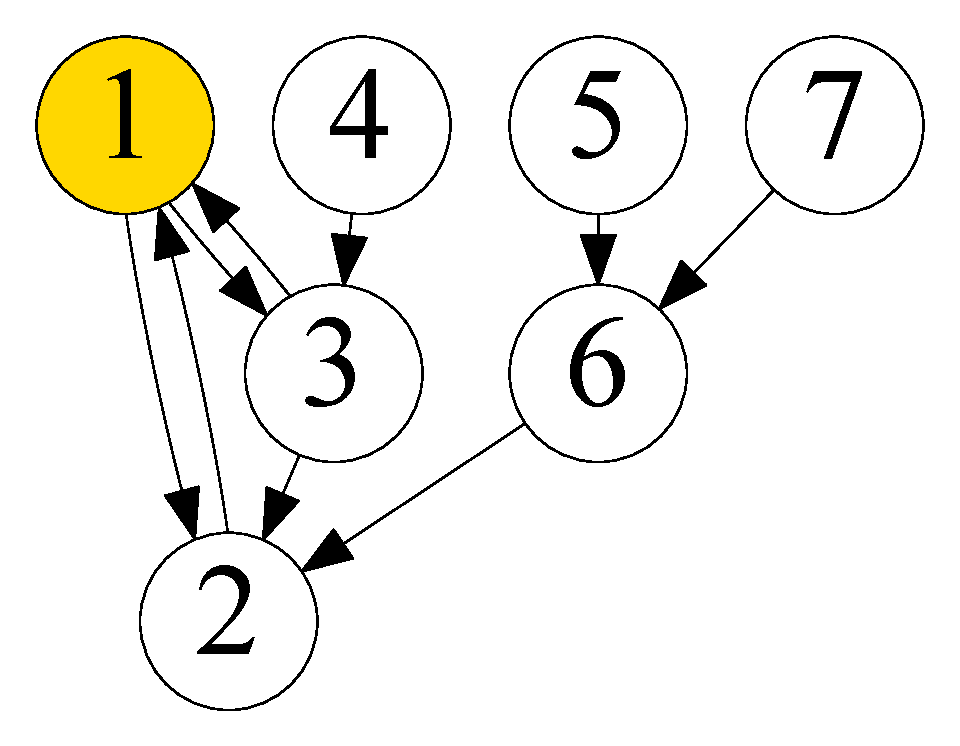
\includegraphics[width=0.3\columnwidth]{./alg_fig/fvs-eg}
\vspace{-1em}
\caption{An example of a directed graph; node 1 forms a feedback vertex set.}
\vspace{-1em}
\label{fig:fvs}
\end{figure}

% dependency graph
%Our algorithms for IBVR are based on a graph representation of the transaction batches. 
Every batch $B$ of viable transactions induces a \emph{dependency graph} $G$; this is a directed graph whose nodes are the transactions in $B$ and whose edges are read-write dependencies.
\eat{
% first show if the graph is acyclic, then we are done
% if the graph is acyclic, we can construct prec
If $G$ is acyclic, then there exists a $\prec$ on $G$ that respects all read-write dependencies; we can construct it as follows. The edges in $G$ provide a strict partial order on $B$; for two nodes $t, t' \in G$, we order $t$ before $t'$ if and only if $t'$ is reachable from $t$ (they cannot both be reachable from each other by acyclicity). We complete the construction of $\prec$  by choosing any linear extension of this partial order.

% if there is a prec, we ensure no violation of read-write depedency exists
We need to show that if $t \prec t'$, then there is no read-write dependency from $t'$ to $t$. Suppose $t \prec t'$ and consider the nodes $t$ and $t'$ in $G$. Assume for a contradiction there is a read-write dependency from $t'$ to $t$. Then by construction, $G$ contains an edge from $t'$ to $t$, and by construction of $\prec$ we have $t' \prec t$; however, this contradicts the statements that $t \prec t'$ and that $\prec$ is strict.

Our family of algorithms for IBVR is based on constructing the dependency graph $G$ and finding a \emph{feedback vertex set} (FVS) on $G$~\cite{karp1972reducibility}. A FVS is a subset of vertices whose removal makes the graph acyclic. For example, consider the graph in Figure~\ref{fig:fvs}. The vertex 1 forms a FVS since the graph becomes acyclic after removing vertex 1 and its incoming and outgoing edges.

Finding a minimal-size $B'$ for IBVR is exactly the problem of finding the minimal (smallest-size) feedback vertex set on $G$. If we have a more complex objective function for IBVR, we can push the objective function into the FVS computation; we assign weights to the nodes to represent the desired transaction priorities, and look for a minimum-weight FVS. 

Once we find the FVS $B'$, removing the nodes in $B'$ from $G$ yields an acyclic graph that allows us to determine the desired serialization order $\prec$.
}% end \eat

If $G$ is acyclic, then there exists a commit order $Q$ on $G$ that respects all read-write dependencies. We can construct $Q$ by repeatedly committing a transaction whose corresponding node in $G$ has no outgoing edge. If $G$ is not acyclic, we can show that the problem is NP-hard by reducing the NP-hard problem of finding a directed feedback vertex set to it~\cite{karp1972reducibility}. 
%This is always feasible when $G$ is acyclic.
%Our family of algorithms for IBVR is based on constructing the dependency graph $G$ and finding a \emph{feedback vertex set} (FVS) on $G$~\cite{karp1972reducibility}. 


A feedback vertex set (FVS) of a directed graph is a subset of vertices whose removal makes the graph acyclic. For example, consider the graph in Figure~\ref{fig:fvs}. The vertex 1 forms a FVS since the graph becomes acyclic after removing vertex 1 and its incoming and outgoing edges. Finding a minimal-size $B'$ for IBVR is exactly the problem of finding the minimal (smallest-size) feedback vertex set on $G$. If we have a more complex objective function for IBVR, we can assign weights to the nodes to represent the desired transaction priorities, and look for a minimum-weight FVS. 
Once we find the FVS $B'$, removing the nodes in $B'$ from $G$ yields an acyclic graph that determines the desired commit order $Q$.


\eat{
\subsubsection{Complexity of FVS}\label{subsec:FVS_stateoftheart}

The directed graph FVS (DFVS) problem is well-studied as it has many applications, including deadlock detection, program verification, and Bayesian inference. 

It was listed among the first set of NP-complete problems~\cite{karp1972reducibility}. 
The state-of-the-art study on the hardness of the problem has shown that it is \emph{fixed-parameter tractable}~\cite{chen2008fixed}, that is, it can be solved in time $O(f(k)n^c)$ for a function $f(k)$ and a constant $c$ where the number $k$ and the function $f(k)$ are independent of the instance size $n$. \cite{chen2008fixed} proposes an exact algorithm for finding a minimal DFVS in $O(4^kk!n^{O(1)})$, where $n$ is the number of vertices and $k$ is the size of the minimal solution. 

DFVS is also APX-hard~\cite{kann1992approximability}. This means there exists a constant $c>1$ such that the existence of a polynomial-time approximate algorithm that achieves an approximation ratio strictly smaller than $c$ would imply $P=NP$. The best hardness result~\cite{dinur2005hardness} shows that it is NP-hard to approximate DFVS within a factor of 1.36, by an easy reduction from vertex cover. While it is still open whether there exists a constant factor approximation for DFVS, it is shown that it is NP-hard to approximate DFVS within any constant factor if the Unique Games Conjecture is true~\cite{guruswami2008beating}. The state-of-the-art algorithm has an approximation factor of $O(\log\tau\log\log\tau)$, where $\tau$ is the size of the exact solution, and a factor of $O(\log\tau^*\log\log\tau^*)$ for weighted directed graphs, where $\tau^*$ is the weight of the exact solution.

Despite the above hardness results, empirical studies have shown that simple greedy heuristics perform reasonably well when compared to more advanced algorithms~\cite{cutello2015targeting}. 
}%end \eat

%We need fast algorithms to avoid increasing both transaction latencies and the number of aborts. 
The directed graph FVS (DFVS) problem is well-studied as it has many applications, including deadlock detection, program verification, and Bayesian inference. It is NP-hard and APX-hard~\cite{kann1992approximability, karp1972reducibility}, and it is still an open problem whether there exists any constant-factor approximation.
We propose two greedy algorithms for finding feedback vertex sets -- one based on the graph's strongly connected components (SCCs) and the other based on sort. We also introduce a hybrid algorithm that makes strategic use of brute-force search, and consequently is slower but more precise.

All our IBVR algorithms begin by constructing the dependency graph $G$. We start with a set of transactions that have been batched at the validator and construct $B$ by discarding all non-viable transactions. We can identify such transactions by validating each transaction against all the updates prior to this batch.
Next, we create one node per transaction, and one edge per read-write dependency. To determine whether a read-write dependency holds from transaction $t'$ to $t$, we check whether $WS(t) \cap RS(t') \neq \emptyset$. If so, we add an edge from $t'$ to $t$. We can implement this by creating a hash table from the write sets and probing it with the read sets. The time complexity of building $G$ is $O(|B|+|R|+|W|)$, where $|B|$ is the size of $B$, $|R|$ is the total number of reads, and $|W|$ is the total number of writes. 

We now process $G$ to find a feedback vertex set. Both before and during the execution of our FVS algorithms, we \emph{trim} the graph to remove all nodes which have no incoming edges and/or no outgoing edges; such nodes cannot participate in any cycles and are unnecessary to include in any FVS.

\eat{
\begin{algorithm}[t]
\caption{SCC-based greedy algorithm}
\label{alg:scc}
\begin{algorithmic}[1]
%\SetAlgoLined\DontPrintSemicolon
%\SetKwProg{main}{Algorithm}{}{}
\Procedure{GreeduSccGraph}{$G$,$P$}
%\main{GreedySccGraph($G$, $P$)}{
%\KwIn{Directed graph $G$, policy $P$}
%\KwOut{$V$, a feedback vertex set for $G$}
\State $V\gets \emptyset$
\State $G'\gets trim(G)$
\State $SCC = StronglyConnectedComponents(G')$
\For {$S \in SCC$} 
	\State $V\gets V\cup GreedyComponent(S, P)$
\EndFor
\Return{$V$}
\end{algorithmic}
\end{algorithm}
}%end \eat

\begin{algorithm}[t]
\SetAlgoLined\DontPrintSemicolon
\SetKwProg{main}{Algorithm}{}{}
\main{GreedySccGraph($G$, $P$)}{
\KwIn{Directed graph $G$, policy $P$}
\KwOut{$V$, a feedback vertex set for $G$}
$V\gets \emptyset$\;
$G'\gets trim(G)$\;
$SCC = StronglyConnectedComponents(G')$\;
\For {$S \in SCC$} {
	$V\gets V\cup GreedyComponent(S, P)$\;
}
\Return{$V$}\;
}{}

\SetKwProg{sub}{Algorithm}{}{}
\sub{GreedyComponent($S$, $P$)}{
\KwIn{SCC $S$, policy $P$}
\KwOut{$V'$, a feedback vertex set for $S$}

\If {$S.size == 1$} {
	\Return{$\emptyset$}\;
}
$V' \gets \emptyset$\;
$v\gets select(S, P)$\;
$V'\gets V'\cup v$\;
$S'\gets delete(S, v)$\;
$V'\gets V'\cup GreedySccGraph(S', P)$\;
\Return{$V'$}\;
}{}

\caption{SCC-based greedy algorithm}
\label{alg:scc}
\end{algorithm}


\begin{algorithm}[t]
\SetAlgoLined\DontPrintSemicolon
\SetKwProg{main}{Algorithm}{}{}
\main{GreedySortGraph($G$, $P$, $k$)}{
\KwIn{Directed graph $G$, policy $P$, multi factor $k$}
\KwOut{$V$, a feedback vertex set for $G$}
$V\gets \emptyset$\;
$G\gets trim(G)$\;
\While {$G\neq \emptyset$} {
	\If {$G.size < k$} {
	 	$V\gets V\cup GreedySortGraph(G, P, 1)$\;
	 	break\;
	}
	$Q\gets sort(G, P)$\;
	\For {$i=1; i\leq k; ++i$} {
		$V\gets V\cup Q[i]$\;
		$G\gets remove(G, Q[i])$\;
	}
	$G\gets trim(G)$\;
}
\Return{$V$}\;
}{}
\caption{Sort-based greedy algorithm}
\label{alg:sort}
\end{algorithm}



%\subsubsection{SCC-based greedy algorithm}

{\bf SCC-Based Greedy Algorithm.} The intuition behind our first algorithm is that each cycle is contained in a strongly connected component of the graph, so we can process the components separately. After preprocessing, we partition the graph into SCCs. For a graph with $V$ vertices and $E$ edges, we can do this in time $O(|V|+|E|)$ using Tarjan's SCC algorithm~\cite{tarjan1972depth}.

Any SCC that consists of a single node does not need to be considered further, as the single vertex involved cannot be on a cycle. For any SCC that consists of more than a single node, we choose a vertex to remove according to some \emph{policy}. The policy is a ranking function over vertices, and we greedily choose the top-ranked vertex to remove. We then recurse on the remaining graph. Algorithm~\ref{alg:scc} shows the details of this procedure. We begin by trimming and partitioning the graph into SCCs  (lines 3-4). We process each SCC $S$ using $GreedyComponent(S, P)$ (lines 5-7). This subroutine starts by eliminating SCCs of size one (lines 10-12). Next, it chooses the top-ranked vertex $v$ from $S$ under Policy $P$ (line 14). It includes $v$ in the $FVS$ of $S$ (line 15), removes it from $S$ (line 16), and it recursively calls $GreedySccGraph$ on the remaining graph (line 17). Finally, it returns the union of all the FVSs obtained in processing $S$ (line 18). When the top-level procedure $GreedyComponent(G, P)$ has processed all the SCCs of $G$, it returns the union of the FVSs obtained (line 8).

The policy $P$ is at the heart of the algorithm, and it affects both its accuracy and runtime. Fortunately, there is no trade-off between accuracy and running time; a more accurate policy will lead to a smaller FVS and faster termination. We discuss possible policies in Section \ref{subsec:validator_reordering:policy}.

%\subsubsection{Sort-based greedy algorithm}

\begin{figure*}[t]
    \centering
    \begin{minipage}[b]{0.19\linewidth}
        \captionsetup{type=figure}
        \centering
        \subcaptionbox{original\label{fig:scc:g0}}
            {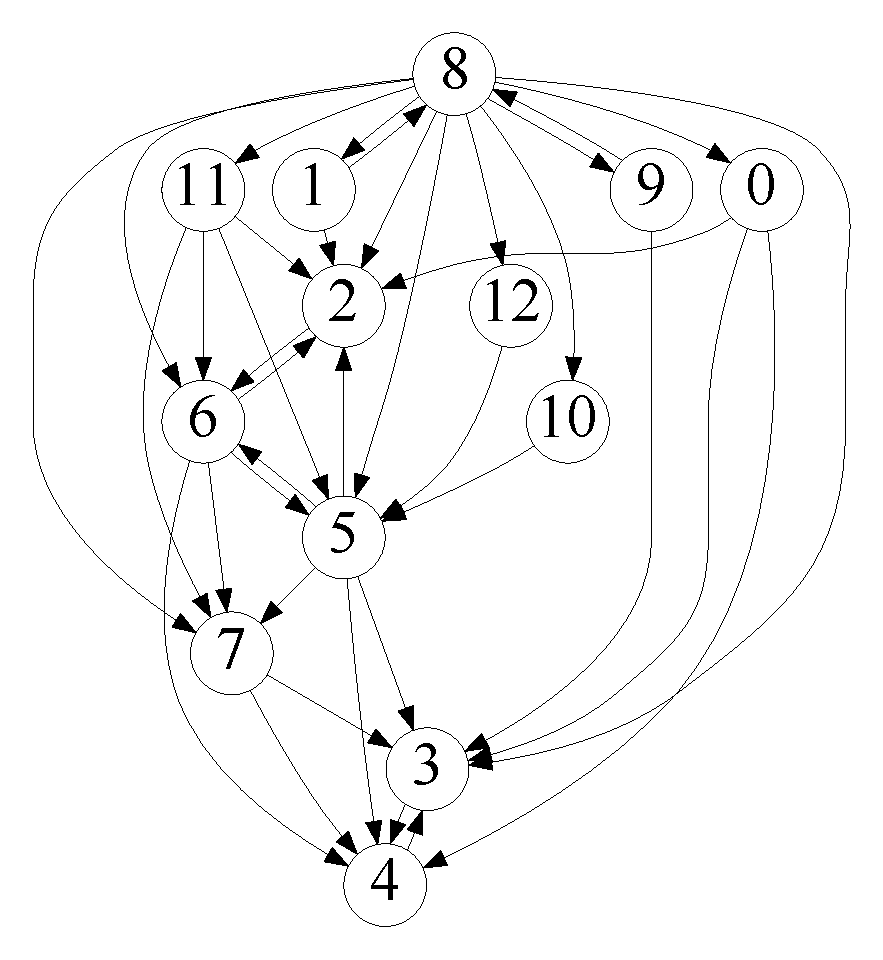
\includegraphics[width=\textwidth]{./alg_fig/scc-g0}}
   %     \vspace{-2em}
    \end{minipage}
   	\begin{minipage}[b]{0.19\linewidth}
        \centering
        \subcaptionbox{partition into SCCs\label{fig:scc:g1}}
                    {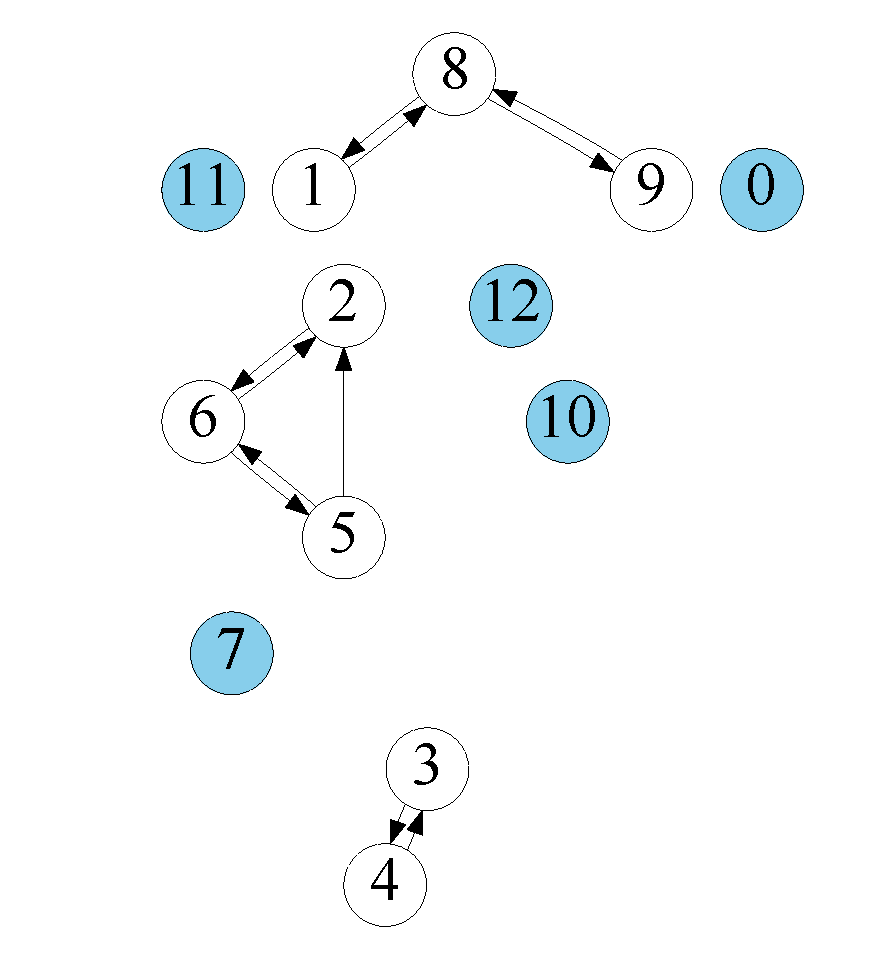
\includegraphics[width=\textwidth]{./alg_fig/scc-g1}}
    %    \vspace{-2em}
    \end{minipage}
    \begin{minipage}[b]{0.19\linewidth}
            \centering
            \subcaptionbox{add 3 to FVS\label{fig:scc:g3}}
                        {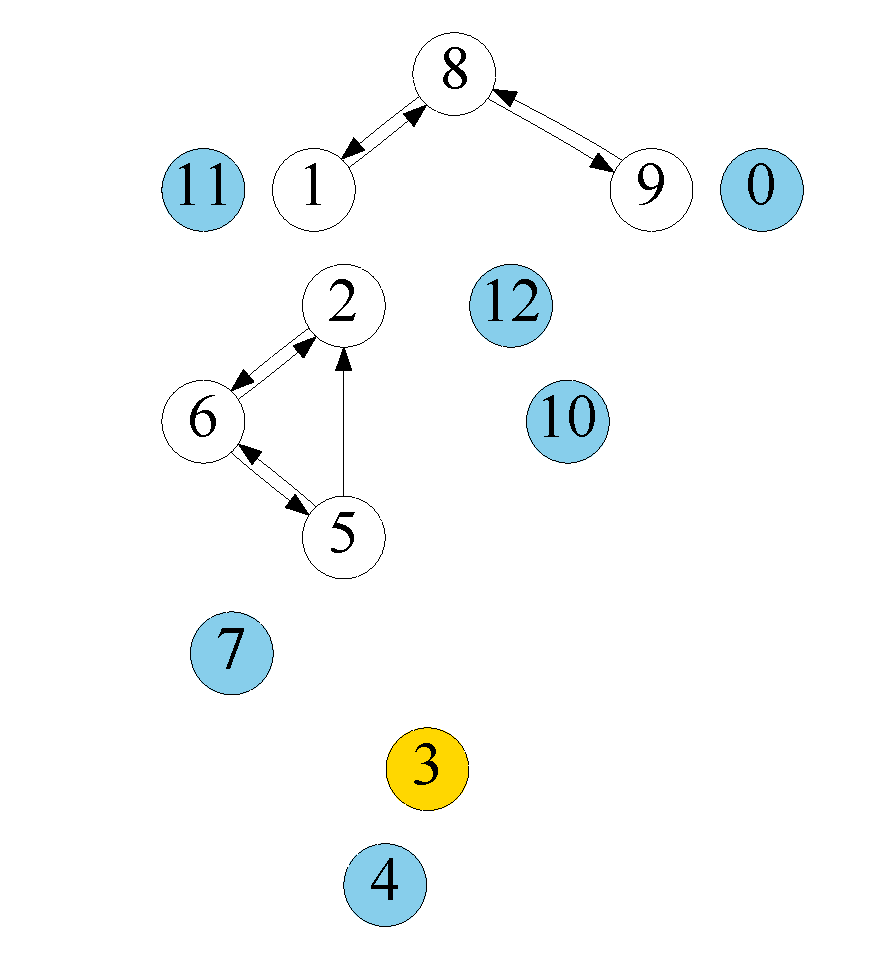
\includegraphics[width=\textwidth]{./alg_fig/scc-g3}}
     %       \vspace{-2em}
        \end{minipage}
    \begin{minipage}[b]{0.19\linewidth}
            \centering
            \subcaptionbox{add 6 to FVS\label{fig:scc:g5}}
                        {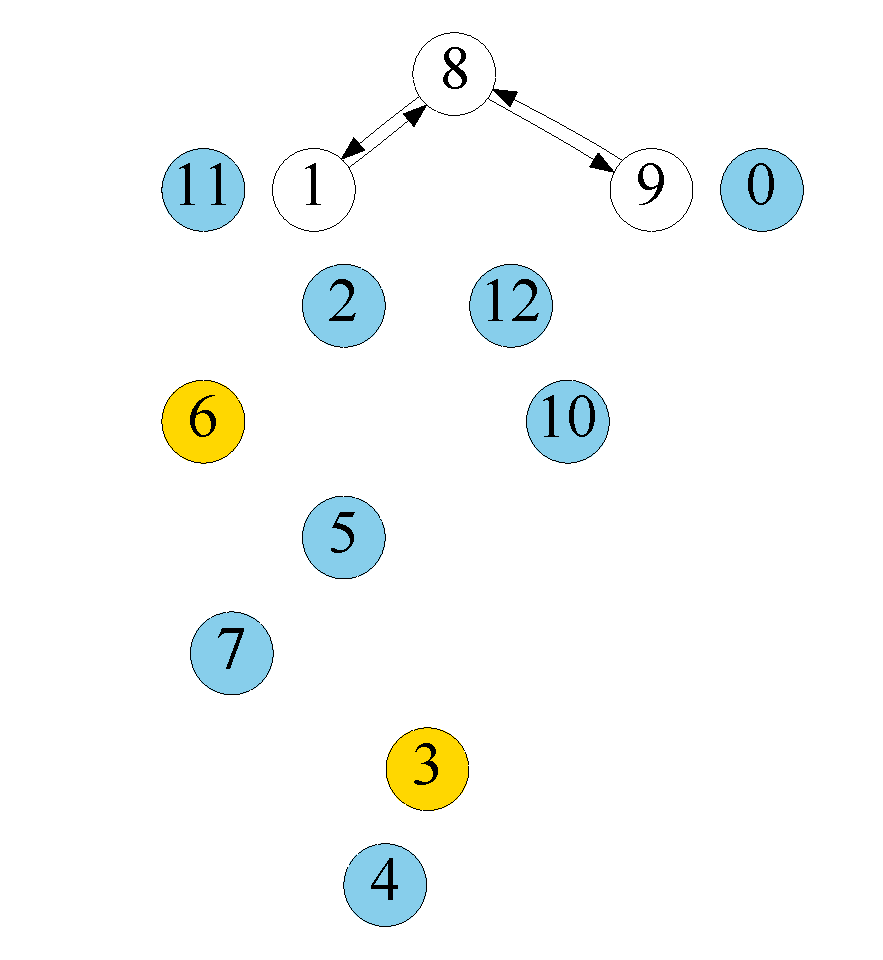
\includegraphics[width=\textwidth]{./alg_fig/scc-g5}}
      %      \vspace{-2em}
   		\end{minipage}                  
    \begin{minipage}[b]{0.19\linewidth}
            \centering
            \subcaptionbox{add 8 to FVS\label{fig:scc:g7}}
                        {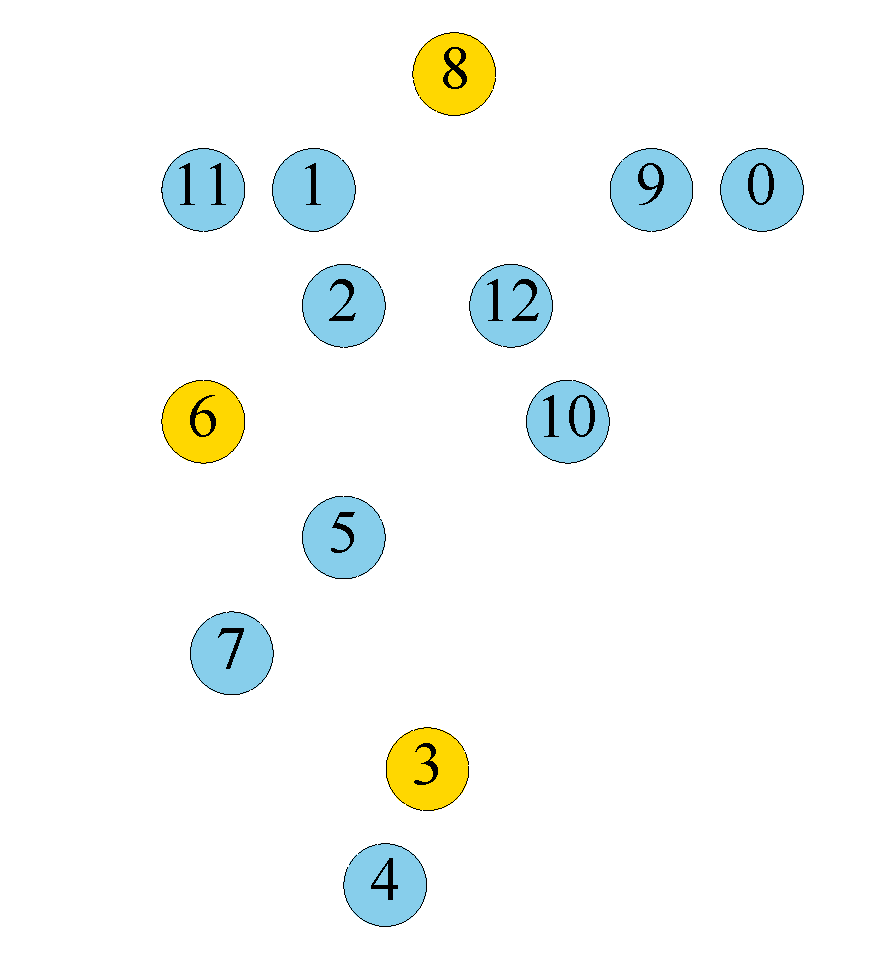
\includegraphics[width=\textwidth]{./alg_fig/scc-g7}}
       %     \vspace{-2em}
   		\end{minipage}  
  	\vspace{-1em}             
   \caption{An example of the SCC-based greedy algorithm using \texttt{prod-degree} policy}
   \vspace{-1em}
   \label{fig:scc}
\end{figure*}


\begin{figure*}[t]
    \centering
    \begin{minipage}[b]{0.19\linewidth}
        \captionsetup{type=figure}
        \centering
        \subcaptionbox{original\label{fig:simple:g0}}
        	{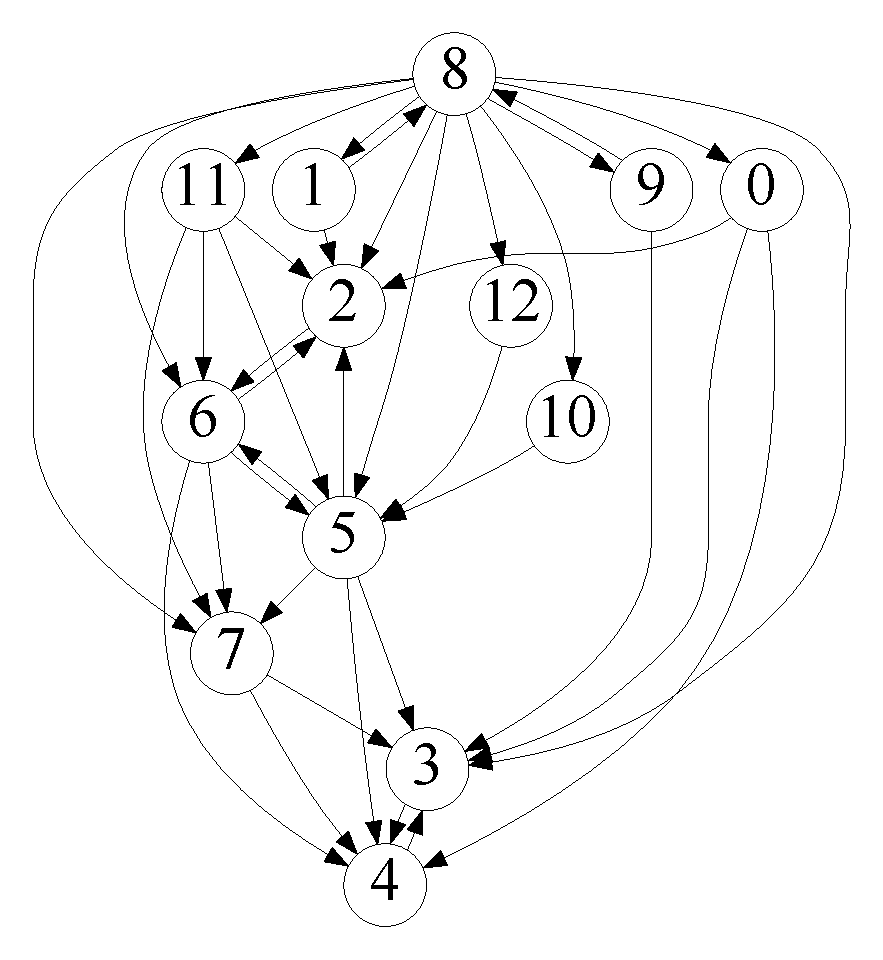
\includegraphics[width=\textwidth]{./alg_fig/simple-g0}}
   %     \vspace{-2em}
    \end{minipage}
    \begin{minipage}[b]{0.19\linewidth}
        \centering
        \subcaptionbox{add 5 to FVS\label{fig:simple:g2}}
        {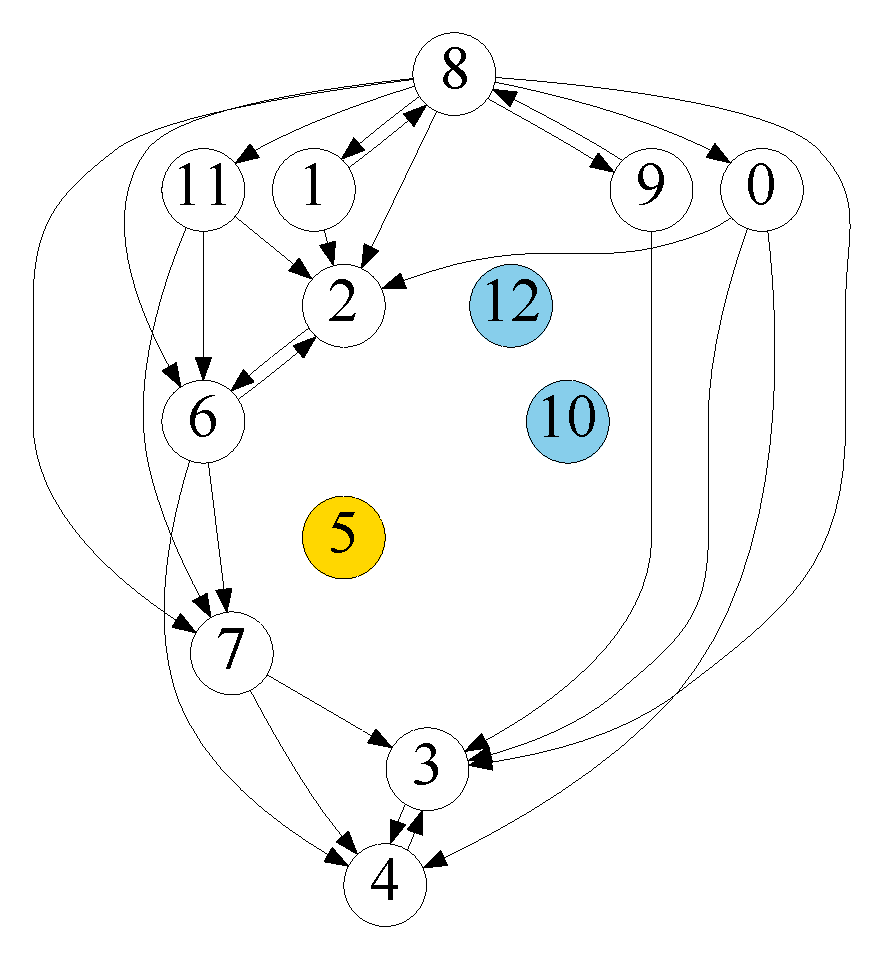
\includegraphics[width=\textwidth]{./alg_fig/simple-g2}}
    %    \vspace{-2em}
    \end{minipage}
    \begin{minipage}[b]{0.19\linewidth}
            \centering
        \subcaptionbox{add 8 to FVS\label{fig:simple:g4}}
            {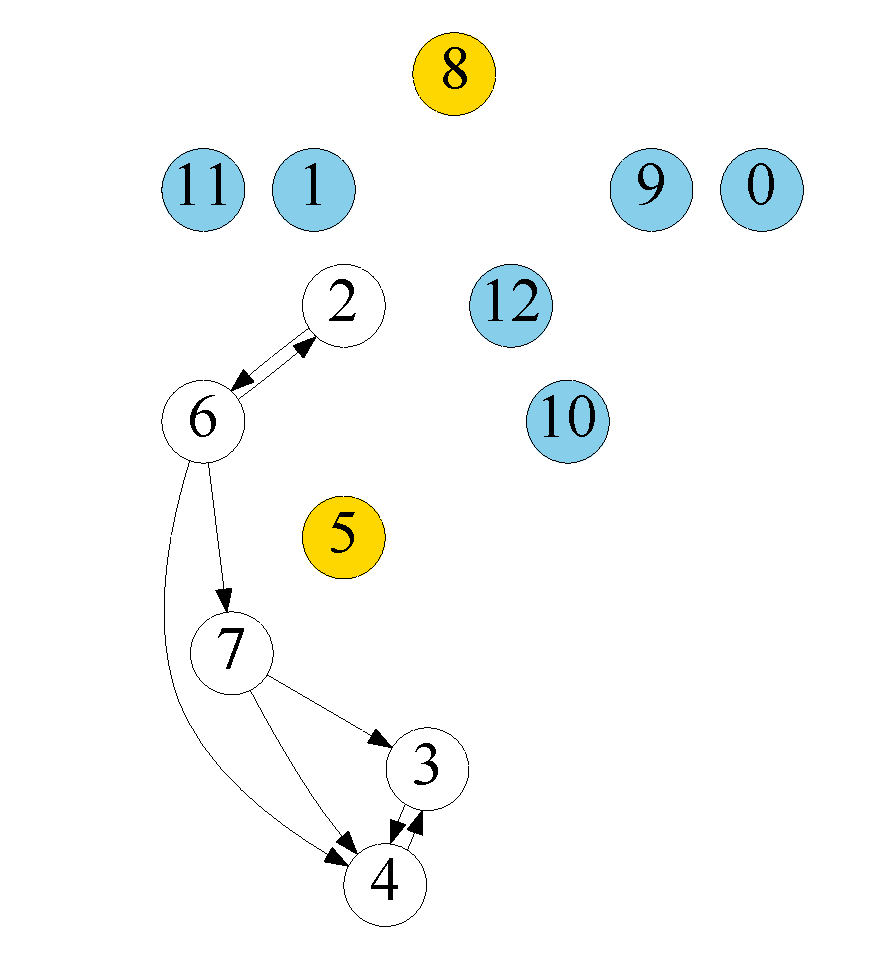
\includegraphics[width=\textwidth]{./alg_fig/simple-g4}}
     %       \vspace{-2em}
        \end{minipage}
    \begin{minipage}[b]{0.19\linewidth}
            \centering
             \subcaptionbox{add 6 to FVS\label{fig:simple:g6}}
			{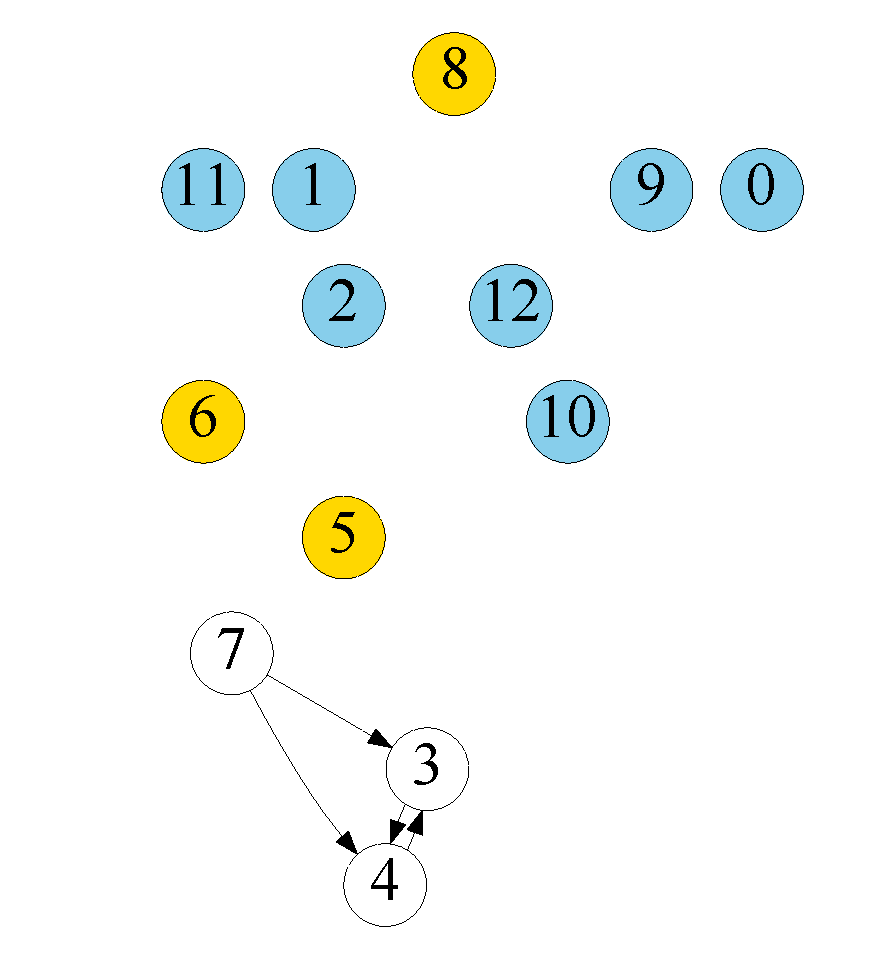
\includegraphics[width=\textwidth]{./alg_fig/simple-g6}}
      %      \vspace{-2em}
   		\end{minipage}                  
    \begin{minipage}[b]{0.19\linewidth}
            \centering
             \subcaptionbox{add 3 to FVS\label{fig:simple:g8}}
            {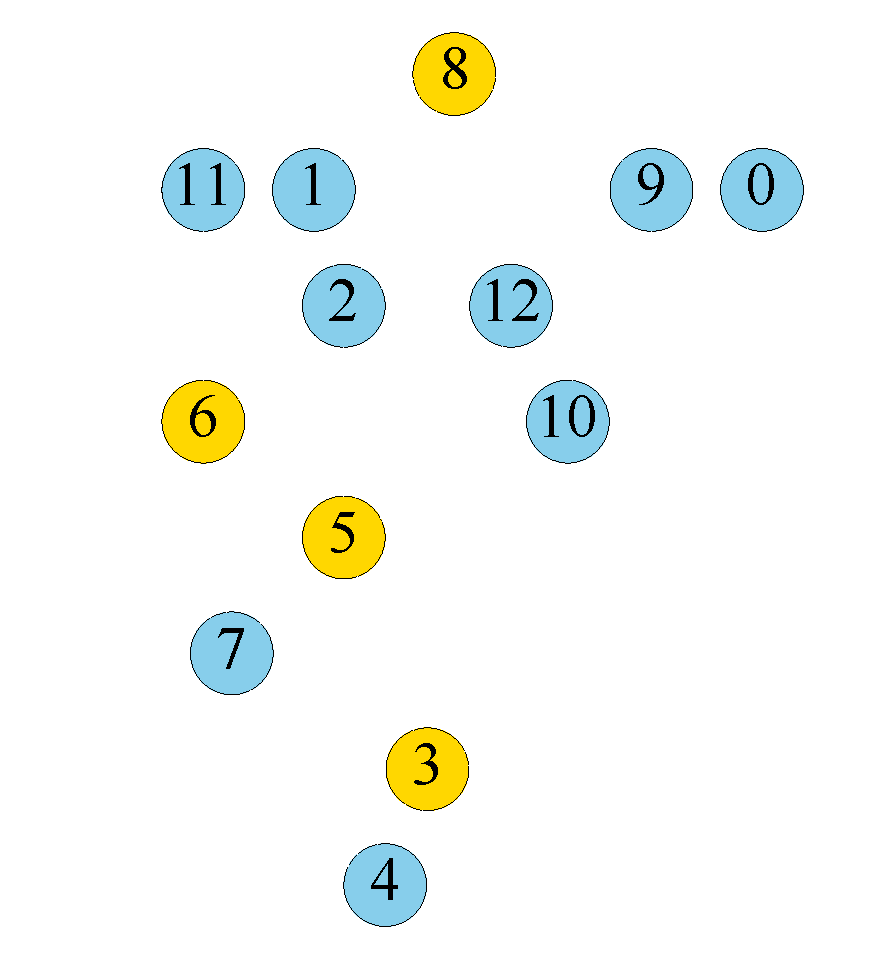
\includegraphics[width=\textwidth]{./alg_fig/simple-g8}}
       %     \vspace{-2em}
   		\end{minipage}
  	\vspace{-1em}             
   \caption{An example of the sort-based greedy algorithm using \texttt{prod-degree} policy and multi factor 1}
   \label{fig:simple}               
   \vspace{-1em}    	
\end{figure*}

{\bf Sort-Based Greedy Algorithm.} Our first algorithm relied on a SCC partitioning routine that takes linear time in the size of the graph. As this routine is called several times throughout the algorithm, it can cause a non-trivial overhead. Here we propose a faster greedy algorithm which uses a sort-based approach to remove nodes. Through extensive empirical tests of the SCC-based greedy algorithm we found that nodes with certain properties are very likely to be included in a FVS. Such nodes generally have high in-degree and/or out-degree. Our second algorithm is based on this observation; it sorts the nodes according to their policy $P$, and includes the top-ranked $k$ nodes in the FVS. We call $k$ the \emph{multi factor} of the algorithm. The algorithm removes these nodes and iterates on the remaining graph.

Algorithm~\ref{alg:sort} shows this in more detail. We trim the graph (line 3); if the graph has no more than $k$ nodes, we reduce the multi-factor to 1 (line 5-8). Otherwise, we sort the nodes into a queue $Q$ using $P$, and include the top-ranked $k$ nodes in $V$ (line 9-13).
After removing the selected nodes from $G$, we trim the remaining the graph again (line 14). We repeat this procedure until the graph is empty (line 4). This algorithm is faster but less accurate than the SCC-based greedy algorithm. However, as we will see in Section~\ref{sec:experiments}, in practice it produces results of comparable accuracy to the SCC-based algorithm.

{\bf Hybrid Algorithm.}
%\subsubsection{Hybrid algorithm} 
We can combine the SCC-based greedy algorithm and the precise brute-force FVS search into a \emph{hybrid algorithm}. The algorithm is similar to the SCC-based greedy algorithm but runs a precise, brute-force FVS search whenever it can afford to. Thus instead of processing all SCCs via the $GreedyComponent$ subroutine (lines 5-7 of Algorithm~\ref{alg:scc}), it runs the precise search when processing SCCs that are smaller than a certain \emph{threshold}, and the greedy subroutine $GreedyComponent$ on SCCs that are larger than the threshold. Adjusting the threshold allows us to trade off precision versus runtime.


\subsection{An Example}\label{subsec:alg_example}

We will illustrate how the two algorithms behave on a simple example. Figures \ref{fig:scc} and \ref{fig:simple} show executions of the two greedy algorithms on the same graph. Both algorithms use a policy where the ranking of a node is the product of its in-degree and its out-degree; we call this policy \texttt{prod-degree}.

Figure~\ref{fig:scc} shows the SCC-based greedy algorithm. The graph cannot be trimmed, so we partition it into SCCs. We remove all SCCs of size 1 --  Nodes 0, 7, 10, 11, and 12 (Figure~\ref{fig:scc:g1}). There are three remaining SCCs. We first look at the component containing Nodes 3 and 4. Since Nodes 3 and 4 have the same product of in-degree and out-degree, we can add either one of them to the FVS. We choose Node 3. Now Node 4 has neither incoming nor outgoing edges, so it is trimmed (Figure~\ref{fig:scc:g3}). We repeat the process with the other components. For the SCC containing Nodes 2, 5, and 6, we add Node 6 to the FVS, as it has the largest product of in-degree and out-degree among the three nodes in this SCC. We now trim Nodes 2 and 5 (Figure~\ref{fig:scc:g5}). Finally, we remove Node 8 from the last component, and trim Nodes 1 and 9 (Figure~\ref{fig:scc:g7}). This leaves us with a final FVS consisting of Nodes 3, 6, and 8.

Figure~\ref{fig:simple} shows the same example using the sort-based greedy algorithm, with $k = 1$. After the first sort, we add Node 5 to the FVS since it has the highest product of in-degree and out-degree. After eliminating Node 5, Nodes 10 and 12 have only incoming edges, and get trimmed (Figure~\ref{fig:simple:g2}). We sort the remaining nodes. This time, we add Node 8 to the FVS, and trim Nodes 0, 1, 9, 11 (Figure~\ref{fig:simple:g4}). We repeat this process with the remaining nodes until the graph is empty. This yields a FVS consisting of Nodes 3, 5, 6, and 8 (Figure~\ref{fig:simple:g8}), which contains one more vertex than the FVS we obtained with the SCC-based algorithm.


\subsection{Incorporating Policies}
\label{subsec:validator_reordering:policy}

Policies are of upmost importance for our algorithms. Recall that a policy is a ranking function on vertices of the graph, and a good policy ranks vertices which are likely to be in a desirable FVS highly. 

We first discuss policies that aim at minimizing the number of conflicts, i.e., the size of the FVS. The simplest such policy is \texttt{random} that assigns all nodes random rankings. Alternatively, we can rank nodes using degree-based heuristics, which use the intuition that the removal of a node will break many cycles if the node is high in some measurement of its graph degree. Such heuristics have  been shown to work well for FVS computation~\cite{cutello2015targeting}. For example, the policy \texttt{max-degree} chooses the node with the largest degree (either in-degree or out-degree), \texttt{sum-degree} chooses the node with the largest total degree (in-degree plus out-degree), and \texttt{prod-degree} chooses the node with the largest product of in-degree and out-degree. 

More sophisticated policies are possible if the system is optimizing a metric beyond maximizing the number of commits. For example, we may want to bound the transactions' tail latency; we can do that by incorporating latency information in our policies. We can rank transactions based on how many times they have been aborted and restarted, breaking ties using degree-based heuristics; thus, transactions that have been restarted many times are less likely to enter the FVS and have a higher chance of committing. While this policy reduces the transactions' tail latency, it can increase the non-tail latency.
%, due to its suboptimality in finding the feedback vertex set. 
To alleviate this problem, we can devise policies that combine information about a transaction's number of restarts and its graph degree. For example, we can compute the ranking of a vertex as the product of its in-degree and out-degree divided by an exponential function of the number of restarts of the corresponding transaction. 

We can also devise policies that handle hard transactions. In many workloads some transactions are naturally more prone to conflicts, e.g., those that access many objects and/or ``hot'' objects. If we use graph degree based policies, such transactions are likely to be included in the FVS and aborted repeatedly. To avoid starvation, we can adjust our policies to increase the probability that these transactions can commit. For example, we can approximate the ``hardness'' of a transaction by the size of its read and write sets and include that as a weighting factor in the policy. 





